\section{Choosing Stairs or the Elevator}
When the algorithm stands between choosing the stairs, or an elevator when traveling to another floor, the choice is determined by the weight of the route. The weight is based on how time consuming or psychical fatiguing the process is for the user. In order to weight the vertex in a way that reflects reality the stairs weight should grow exponentially. The more stairs a user climbs in succession the more psychical fatiguing it gets which is the reasoning for the exponential growth. This have however been delimited 
%(indsæt_smart_reference_til_afgrænsing_her)
 and both the stairs and elevator will therefore be weighted in a linear manner. The figure \cref{labeled_stairsVSelevators} shows a graph with the stairs and elevator. The elevator starts with more initial weight as it takes time to enter the elevator and select a floor to go to, where the stairs start ascending as soon the user is on the first step. But once the user is inside the elevator, and it starts ascending, it will catch on the stairs and eventually become the fastest way of traveling. On the graph, the point were the elevator is faster than the stairs, is were the two lines cross, which in this case is between the fourth and third floor. This means if the user has to travel four or more floors, the planned route should utilize the elevator.
\begin{figure}[ht!]
    \centering
    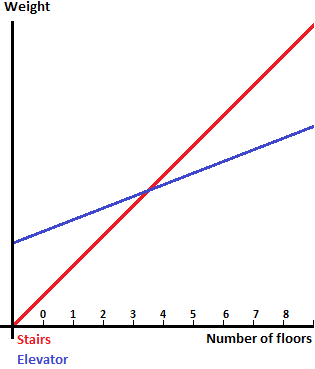
\includegraphics[width=0.5\textwidth]{stairsVSelevators.png}
    \label{fig:labeled_stairsVSelevators}
  \end{figure}
  \end{figure}
  \end{figure}
  \annote{Kapitler er ikke færdigt da det mangler at blive gennemlst, rettet og gennemtænkt. Dett er version 0.8}

  In Stakeholders user, are different people have been described each with their own characteristics, and some people don't have the opportunity to take the elevators or the stairs, to resolve this problem are the weight of a stair or an elevator multiplied with an extremely high number, when the search algorithm travels through the graph then it wont consider e.g. the stairs if the user selected that they would not take the stairs, the same with the elevator. Another way of resolving the problem is to stop the algorithm from considering the stairs by disabling it, if the user choses not to take the stairs, this will make it unusable for the algorithm. A problem with this is if the only way up, is by stairs and the user did selected not to take the stairs, then the program with exit with an error, but if the weight is multiplied with a number, then the search algorithm will take the stairs as an last resort. If the project was to deliver an final product, the program will still show the user the determined route, but prompt the user with a warning.
